\section{Input and Output}
The PCB contains a microcontroller used to manage all input and output between the FPGA and the IO devies shown in figure ~\vref{figure:system-overview}.
The microcontroller listens on all IO channels for input, and acts on the input, either forwarding the request to another device or performing memory operations on the FPGA's memory.

\subsection{Initial requirements}
The assignment required a microcontroller to handle IO for the FPGA.
To minimize the amount of things that could go wrong, much of the initial work was focused on finding a few reliable and relatively simple data connections.

Specifically, the microcontroller was required to be able to put some program and data on the FPGA's memory, and then later output values from the data memory through the proper communication lines.
The I/O devices together with the microcontroller and it's software should be able to provide a reliable and stable I/O connection between the outside world and the FPGA.

\subsection{Communication channels}
\subsubsection{SD Card}
The SD card reader is primarily used as a storage for programs that are to be uploaded on the FPGA.
However, it might also be used to store memory snapshots in order to look how the genetic algorithm converges to a solution over time.

The Energy Micro Application Note on Fat and SD cards, and its example code, describes an implementation of the FatFS library on the Giant Gecko microcontroller.\cite{an0030}

\paragraph{FatFS}\cite{fatfs-web}

FatFS is a generic FAT file system for microcontrollers, with a generic interface for the FAT operations, and a hardware specific interface for disk I/O.
Because of this structure, the system is easily portable.
To add read and write a FAT system on some disk drive, FatFS needs the following functions:

\begin{table}[H]
    \begin{tabular}{| l | l |}
        \hline
        disk\_initialize & Initialize disk drive \\
        \hline
        disk\_status & Get disk status \\
        \hline
        disk\_read & Read sectors on disk \\
        \hline
        disk\_write & Write sectors on disk \\
        \hline
        disk\_ioctl & Control device dependent features \\
        \hline
        get\_fattime & Get current time for FAT \\
        \hline
    \end{tabular}
    \caption{Overview of disk I/O functions}
\end{table}

\subsubsection{USB}
The USB is the main communication line with a host computer, allowing the host computer to start running programs on the FPGA and recieve snapshots of the memory periodically.
The microcontroller has a built in USB controller~\cite{efm32gg990-datasheet} and energy micro has supplied an application note~\cite{an0065} with code for utilizing the included USB controller in order to act as a USB device.

\subsubsection{Serial}
The serial port is meant as a backup solution in case USB doesn't work, with the exact same opportunities, but with an older, simpler interface.
The microcontroller used in the project has a built in UART Receiver/Transmitter\cite{efm32gg990-datasheet} which is easily activated with code from AN0045~\cite{an0045}.

\subsubsection{LEDs and buttons}
The most primitive form of IO we have are the onboard LEDs and buttons.
They allow a quick and easy way to verify that a program is running, and possibly letting the user change execution modes or the program on the FPGA with the buttons.
All code interfacing with the LEDs and buttons are simple code either setting or reading the value of GPIO pins.
The leds are driven by General Purpose IO pins on the SCU, requiring a minimal amount of code in order to get a working output, which is especially handy in the early stages of implementation.

\subsubsection{FPGA}
There are 41 wires between the FPGA and the SCU in order to facilitate communication (see table~\ref{tab:scu-fpga-link} for a complete list of all the connections).
The FPGA has no way of signalling that it wants to output something, so the SCU is responsible for periodically halting the CPU on the FPGA and reading from it's memory.

\subsubsection{J-link}
In order to program and debug the programs on the SCU, we utilize the built-in pins for debugging using J-Link\texttrademark as described in AN0043~\cite{an0043}.
It can also be used as a form of last resort emergency output as it makes it possible to display text that is printed by the program running on the SCU.

\section{FPGA Control}
The only way of communication with the FPGA is with direct memory access to the FPGA's data and instruction memory.
All the data is transfered directly over the SCU's GPIO pins, without any form for memory mapping or built-in bus interfaces.
This is mostly due to the fact that we did not do enough research early in the design process and recognised that we could use something like External Bus Interface to access the memory.

Access to the FPGA's memory is controlled by the signals seen in table~\ref{tab:scu-fpga-link}.
It should be noted that there are two states to access the FPGA's instruction memory, the upper and lower half.
This is because the instruction memory stores 32 bits per address while the SRAM chips only stores 16 bits per address (see section~\ref{subsec:fpga-instruction-memory} for more details on the instruction memory).

The SRAM datasheet~\cite{sram-datasheet} specifies that the data signal has to be stable for at least 10ns in order to complete a write.
This means that it is not necessary to worry about timing when accessing the SRAM since changing the signal more than every 10ns requires a clock speed of 100MHz since we can at most change the ouput of a single pin every cycle.

\begin{table}[H]
    \begin{tabular}{| l | l | l |}
        \hline
        Signal & Bus width & \\
        \hline
        FPGA enable & 1 & Enables the FPGA on high, disables it on low\\
        \hline
        FPGA State & 2 & \pbox{20cm}{00: Processor enable\\01: Instruction memory upper half access\\10: Instruction memory lower half access\\11: Data memory access}\\
        \hline
        Chip enable & 1 & The chip enable signal in to the selected memory block.\\
        \hline
        Write enable & 1 & The write enable signal in to the selected memory block.\\
        \hline
        Address & 19 & The adress bus to the selected memory block.\\
        \hline
        Data & 16 & The data bus to the selected memory block.\\
        \hline
        LBUB & 1 & The LB and the UB signal to the selected memory block.\\
        \hline
    \end{tabular}
    \label{tab:scu-fpga-link}
    \caption{Lines between the SCU and FPGA}
\end{table}

\section{IO Program}
\begin{figure}[H]
    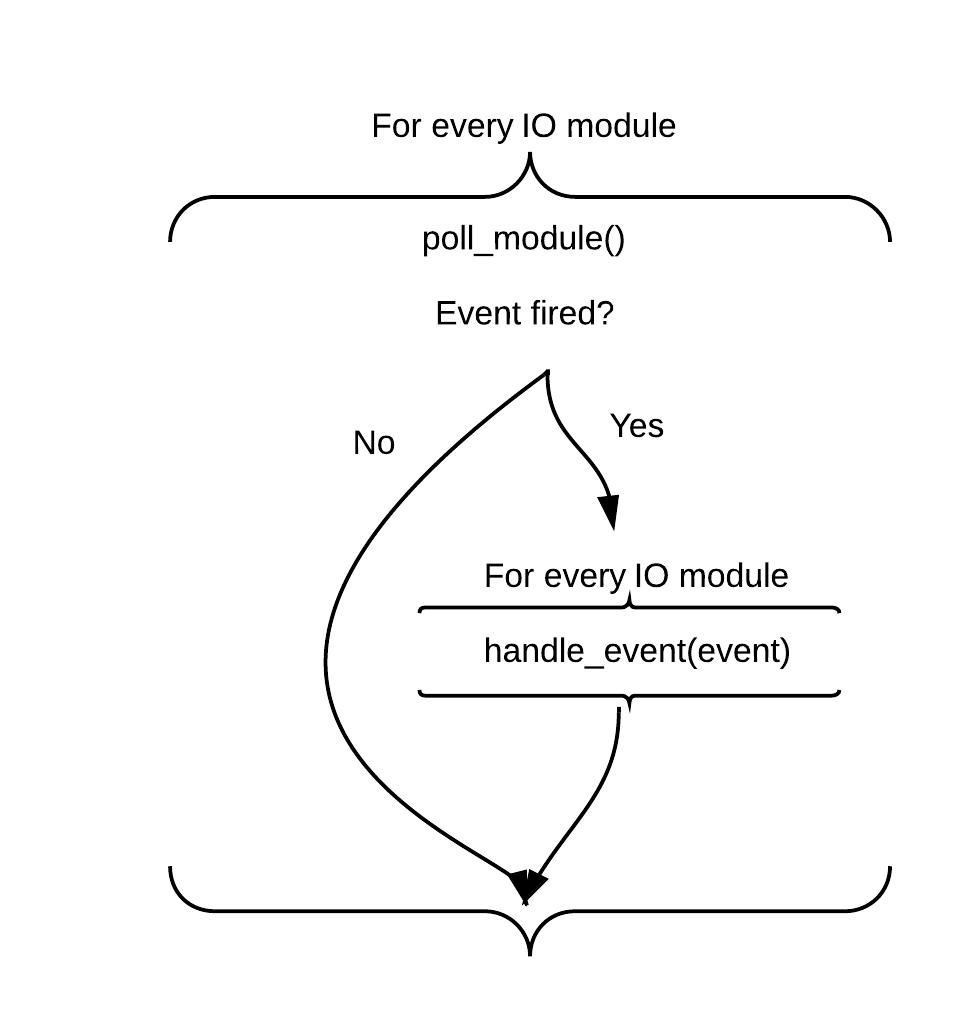
\includegraphics[width=\textwidth]{io/fig/program.png}
    \caption{The body of the IO program's main loop}
\end{figure}

The IO program was designed to be as simple as possible in order to decrease the amount of things that could go wrong.
The main idea is that every IO device is required to define two functions in order to be used: a function to poll for input and a function that is called whenever a device reports input.

In order to enable sending messages between different IO units, the poll functions return a pointer which may point to any object in memory, which allows other modules to read the data given that they know what type of data the pointer points to.

\section{Design decision}
\subsection{Selection of microcontroller}
The microcontroller chosen was chosen as it was the microcontroller we had available to test with on the development kit.
It was also the microcontroller with most available GPIO pins for the package we had to use, which would give us the most possibilities for communication.

\subsection{Operating system}
Early in the process, a discussion arised about how it could be beneficial to run an operating system on the microcontroller such that familiar programs could be run directly on it.
A scenario pitched was to have network access, and then be able to talk to the machine remotely using programs such as \textit{SSH} or \textit{telnet}.
However, the Linux distribution available for the Energy Micro microcontroller was found lacking in the features we wanted, and the microcontroller lacks network support.
It was therefore decided that running an OS was unnecessary as there were few rewards and little to gain from it.

\subsection{FPGA Communication}
During the initial design phase, the link between the FPGA and SCU was designed to be as simple as possible.
The final version was the the 41 wires mapping all the signals needed for directly accessing the SRAM chips.
\todo{Make up some reasons here, should probably defend not using EBI}

\section{Issues}
\subsection{Crystal}
In the design phase it was decided to go with just a single high frequency crystal oscillator.
Unfortunately the crystal that was selected had a clock frequency in the kHz range, instead of the MHz range, which was what was inteded.
Luckily the microcontroller has a built-in RC oscillator, so the crystal oscillator was not essential to get code running on the microcontroller.

\subsection{USB Circuitry not working}
While mapping the PCB curcuitry, only the pins available for GPIO were included initially, but this did not include the vbus and vregi pins.
The pins were connected to capacitors, and a quick hack soldering the appropriate lines to the USB header was tried without success.

\subsection{No UART}
The microcontroller believes that data is being outputted and calls the data sent callback function.
There also seems to be a signal going out to the RS-232 interface, but there is no data being recieved on the other end.

\subsection{Memory access}
\todo{Diagnostics, possibly not just here/not here at all.}
Tried:
\begin{itemize}
    \item Adding delays
    \item Reading immediately after write to verify write,
    \item Mapping control signals to LED on FPGA to verify that they work
    \item Flashing the instruction memory on the FPGA so we just have to read data memory, not write
\end{itemize}
